\subsubsection{External Interface Requirements}
\begin{table}[]
\centering
\caption{User Information}
\label{my-label}
\resizebox{\textwidth}{!}{%
\begin{tabular}{|l|l|}
\hline
Name                                                            & User information                                                                                                                                                                                                                             \\ \hline
Description                                                     & This is information about the user such as Age, Weight, Height and Identification,variables                                                                                                                                                  \\ \hline
\begin{tabular}[c]{@{}l@{}}Source\\ \& Destination\end{tabular} & \begin{tabular}[c]{@{}l@{}}Source:\\ Server, Destination: Device/Application\end{tabular}                                                                                                                                                    \\ \hline
\begin{tabular}[c]{@{}l@{}}Range,\\ accuracy\end{tabular}       & The range of this data : ID (0-60000), Age(0-120),Weight(20-500),Height(20-300)                                                                                                                                                              \\ \hline
\begin{tabular}[c]{@{}l@{}}Unit\\ of measure\end{tabular}       & ID: Integer,,Age: Integer, Weight: kilograms, Height: centimeters                                                                                                                                                                            \\ \hline
Timing                                                          & \begin{tabular}[c]{@{}l@{}}The information will be kept on device until such a point that the user logs out or\\ uninstalls. The Information will be kept on server until such a point that the\\ user deletes his/her account.\end{tabular} \\ \hline
\begin{tabular}[c]{@{}l@{}}Relations\\ to other\end{tabular}    & \begin{tabular}[c]{@{}l@{}}This data relates to the ‘Fitness Information’ data because they are used in the\\ calculations of the fitness statistics.\end{tabular}                                                                           \\ \hline
\begin{tabular}[c]{@{}l@{}}Data\\ format\end{tabular}           & \begin{tabular}[c]{@{}l@{}}This data relates to the ‘Fitness Information’ data because they are used in the\\ calculations of the fitness statistics.\end{tabular}                                                                           \\ \hline
\end{tabular}%
}
\end{table}

\begin{table}[]
\centering
\caption{Navigational Information}
\label{my-label}
\resizebox{\textwidth}{!}{%
\begin{tabular}{|l|l|}
\hline
Name                                                            & Navigational Information                                                                                                                                                                                                                                                                                         \\ \hline
Description                                                     & This is the,navigational data that allows the user to navigate around campus. More,specifically with regards to fitness this data will allow us to keep track of,distances and allow fitness statistics to be drawn from the distances,travelled during navigation                                               \\ \hline
\begin{tabular}[c]{@{}l@{}}Source\\ \& Destination\end{tabular} & Source:Server, Destination: Device/Application                                                                                                                                                                                                                                                                   \\ \hline
\begin{tabular}[c]{@{}l@{}}Range,\\ accuracy\end{tabular}       & \begin{tabular}[c]{@{}l@{}}The range of this information would be roughly (0-100km) as an estimate of the\\ absolute maximum someone would walk in a single day on campus.\end{tabular}                                                                                                                          \\ \hline
\begin{tabular}[c]{@{}l@{}}Unit\\ of measure\end{tabular}       & The unit of,measure for this specific data would be in kilometers                                                                                                                                                                                                                                                \\ \hline
Timing                                                          & \begin{tabular}[c]{@{}l@{}}The information will be kept on device until such a point that the user logs out or\\ uninstalls. The Information will be kept on server until such a point that the\\ user deletes his/her account.\end{tabular}                                                                     \\ \hline
\begin{tabular}[c]{@{}l@{}}Relations\\ to other\end{tabular}    & \begin{tabular}[c]{@{}l@{}}This information relates to ‘fitness information’ because the distances travelled\\ during navigation are to be used in calculating the number of steps made and is\\ crucial in the calculations of calories burned and other fitness statistics\\ that are calculated.\end{tabular} \\ \hline
\begin{tabular}[c]{@{}l@{}}Data\\ format\end{tabular}           & The format,of this would be stored in a float value as to allow accuracy of distances,travelled and would be transferred over JSON as to integrate with our chosen,technology of using Cordova                                                                                                                   \\ \hline
\end{tabular}%
}
\end{table}

\begin{table}[]
\centering
\caption{Fitness Information}
\label{my-label}
\resizebox{\textwidth}{!}{%
\begin{tabular}{|l|l|}
\hline
Name                                                            & Fitness information                                                                                                                                                                                                                                                                                                                                                                        \\ \hline
Description                                                     & \begin{tabular}[c]{@{}l@{}}This is information that is calculated using\\ user information and navigational information and is presented to the user as\\ statistical data of fitness\end{tabular}                                                                                                                                                                                         \\ \hline
\begin{tabular}[c]{@{}l@{}}Source\\ \& Destination\end{tabular} & Source: Application/Device, Destination :Server                                                                                                                                                                                                                                                                                                                                            \\ \hline
\begin{tabular}[c]{@{}l@{}}Range,\\ accuracy\end{tabular}       & \begin{tabular}[c]{@{}l@{}}The range of this data is : DayStep(0-100,000) ,\\ DayCalories(0-10000) DayHeight(0-10000) as maximum that one would be able to\\ walk, burn or climb in a single day.\end{tabular}                                                                                                                                                                             \\ \hline
\begin{tabular}[c]{@{}l@{}}Unit\\ of measure\end{tabular}       & DayStep:,Integer, DayCalories: Calories, DayClimb: Meters                                                                                                                                                                                                                                                                                                                                  \\ \hline
Timing                                                          & The information will be kept on device,until such a point that the user logs out or uninstalls. The Information will,be kept on server until such a point that the user deletes his/her account.                                                                                                                                                                                           \\ \hline
\begin{tabular}[c]{@{}l@{}}Relations\\ to other\end{tabular}    & \begin{tabular}[c]{@{}l@{}}This information is related to user information\\ as the user information is required to determine the fitness statistics. It is\\ also related to navigational data because the distances measured in\\ navigational data are used for the step count and the calories burned as well\\ as determining how high the user has climbed in that day.\end{tabular} \\ \hline
\begin{tabular}[c]{@{}l@{}}Data\\ format\end{tabular}           & \begin{tabular}[c]{@{}l@{}}This information is related to user information\\ as the user information is required to determine the fitness statistics. It is\\ also related to navigational data because the distances measured in\\ navigational data are used for the step count and the calories burned as well\\ as determining how high the user has climbed in that day.\end{tabular} \\ \hline
\end{tabular}%
}
\end{table}

\subsubsection{Performance Requirements}
\begin{enumerate}
	\item Tracking Information Accuracy
	\newline
	The tracking information that is obtained from the Navigation module needs to be as accurate as possible. This will ensure that the information calculated by the fitness module will be accurate and ensure that the user is presented with information that is not false.
	\item Server Storage
	\newline
	The information obtained from other modules and calculated inside the fitness module is to be stored on the server hosting the NavUP application. This means that the server will need to store certain fitness statistics and health information for roughly 60 000 users. The information will need to be able to be stored in a concurrent manner as to not create performance delays during application use.
	\newline
	By storing the fitness information on the server rather than keeping it on the handheld device, we avoid complications whereby the user might uninstall and reinstall the application. Situations whereby the user gets a new phone or performs any actions where there may be data loss can be dealt with in this manner because then information can be re-downloaded.  
	\newline
	By storing fitness information on the server we can also provide a future integration where health-insurance companies could link to the database and use the information to provide some form of a reward system for the user based on his/her fitness achievements.  
	
	\item The User Experience 
	\newline
	All calculations with regards to fitness statistics and other fitness information is to be done on the device itself rather than using the application server. This will relieve the server of traffic and avoid a congested wireless network on campus. The user experience, with regards to local device calculations needs to be perceived as smooth and not be delayed by the calculations.
	
	\item Communication transfer from phone to server
	\newline
	Information transfer between the phone and the server is required to happen in a timely manner when the user requests to calculate fitness information. If the information were to take too long to be retrieved from the server to the phone then the user would have to wait longer than expected to see the fitness information.
	\newline
	With these requirements of fast data transfers there becomes an inherent requirement with regards to the data being sent and retrieved. The data would have to be stored in a format of minimal size as to optimize the fore-mentioned process.
	
	
	\item Reporting of fitness information
	\newline
	The reporting part of the fitness module would need to be able to summarize, format and display certain information in a timely manner as to not delay the user interface thread. This would occur when the user selects the option to view his/her fitness information.
	
\end{enumerate}

\subsection{Design Constraints}

\subsubsection{Software Constraints}
\begin{enumerate}
	\item Device Accelerometer Support:
	\newline
	Given that a device does has an accelerometer, the device manufacturer must provide a software interface to interact with the device's accelerometer.
\end{enumerate}

\subsubsection{Hardware Constraints}
\begin{enumerate}
	\item Accelerometer:
	\newline
	Not all devices models are made equal. Some older devices do not have accelerometers to track steps with. The accuracy of accelerometers also vary from different device manufacturers.
	\item Battery Life:
	\newline
	To track steps continuously with a background process will greatly impact the battery life of devices with small battery capacities. 
\end{enumerate}

\subsection{Software System Attributes} 
\subsubsection{Reliability} 
The fitness module must be able to accurately and reliably track movement through the devices accelerometer. This accuracy and reliability ensures that the calculation of steps, calories and other health related data is accurate. The accuracy and reliability requirements are to ensure that milestones and awards are distributed accurately.    

\subsubsection{Efficiency} 
In order for the application to efficiently count steps and calculate other health metrics, the fitness module needs efficient algorithms to calculate the steps and other health metrics quickly from the data it receives from the accelerometer.  

\subsubsection{Portability} 
The fitness module should be able to work on both iOS and Android devices. There should also be no discernible differences between the fitness module on iOS and the fitness module on Android devices. They should also yield the same the same health metrics. 

\subsubsection{Coupling} 
The fitness module should also integrate with the user module. It should be able to request the users age and name. The fitness module should also be able to write data such as the users height and weight. Minimal health metrics should also be sent to the user module to be stored on the server. 

\subsection{Class Diagram}
See figure~\ref{fig:Fitness_Class_Diagram} on page~\pageref{fig:Fitness_Class_Diagram}
\begin{figure}
	\centering
	\includegraphics[scale=0.54]{Fitness/fitness_class_diagram.png}
	\caption{Fitness Class Diagram}
	\label{fig:Fitness_Class_Diagram}
\end{figure}

\subsection{Design Patterns Used}
\paragraph{Facade}
To provide a simple interface to use the fitness module. The FitUser class inherits from the user class but also provides an interface for the rest of the Fitness Module. The fitCounter, fitCalculator, and fitReport abstract the more complex functions away from the fitUser.

\subsection{Activity Diagram}
See figure~\ref{fig:fitness_activity_diagram} on page~\pageref{fig:fitness_activity_diagram}
\begin{figure}
	\centering
	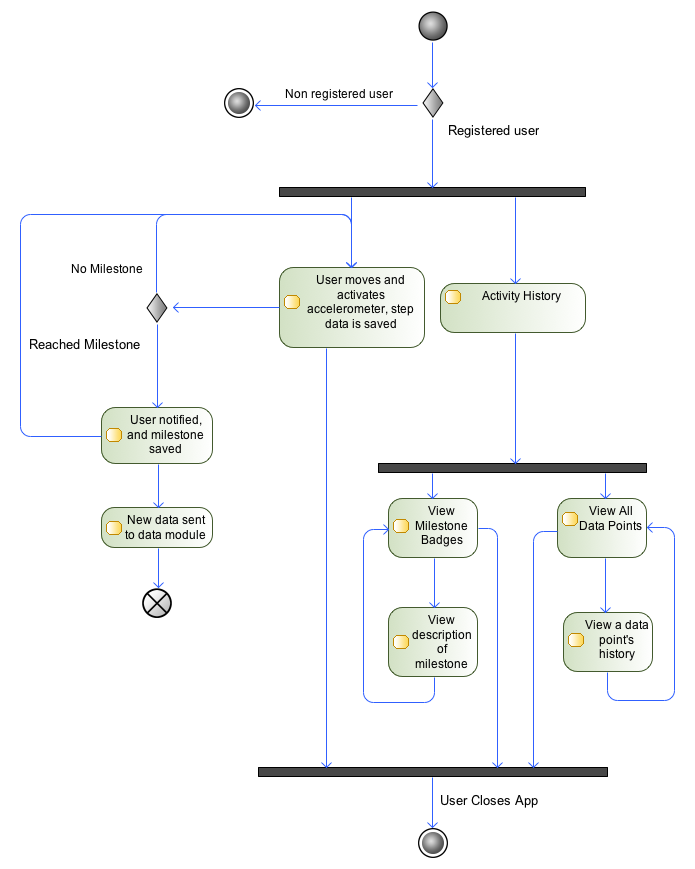
\includegraphics[scale=0.54]{Fitness/fitness_activity_diagram.png}
	\caption{Fitness Activity Diagram}
	\label{fig:fitness_activity_diagram}
\end{figure}

\subsection{Sequence Diagram}
See figure~\ref{fig:Fitness_Sequence_Diagram} on page~\pageref{fig:Fitness_Sequence_Diagram}
\begin{figure}
	\centering
	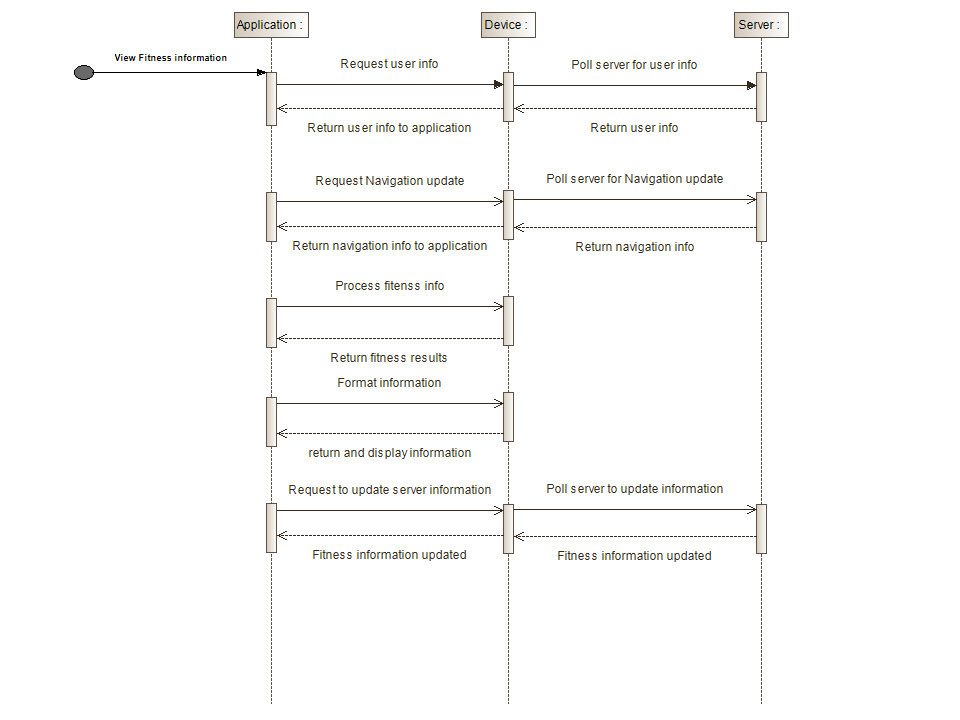
\includegraphics[scale=0.70]{Fitness/fitness_sequence_diagram.png}
	\caption{Fitness Sequence Diagram}
	\label{fig:Fitness_Sequence_Diagram}
\end{figure}

\subsection{State Diagrams}
See figure~\ref{fig:fitness_state_diagram} on page~\pageref{fig:fitness_state_diagram}
\begin{figure}
	\centering
	\includegraphics[scale=0.54]{Fitness/fitness_state_diagram.png}
	\caption{Fitness State Diagram}
	\label{fig:fitness_state_diagram}
\end{figure}

\subsection{Use Case Diagram}
See figure~\ref{fig:Fitness_Use_Case_Diagram} on page~\pageref{fig:Fitness_Use_Case_Diagram}
\begin{figure}
	\centering
	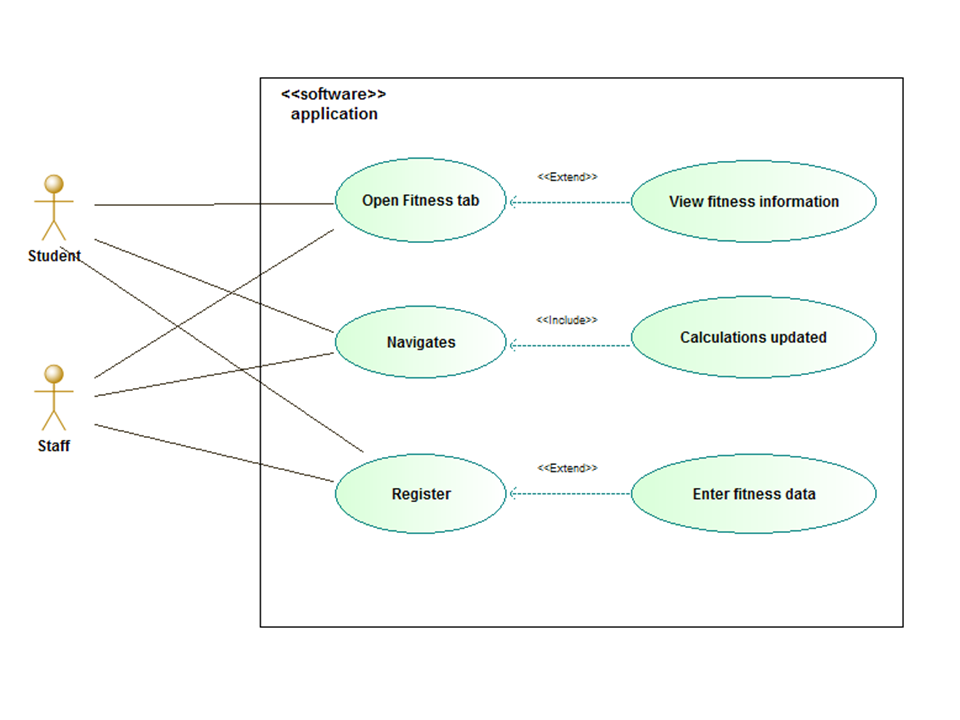
\includegraphics[scale=0.54]{Fitness/fitness_use_case_diagram.png}
	\caption{Fitness Use Case Diagram}
	\label{fig:Fitness_Use_Case_Diagram}
\end{figure}

